\documentclass[12pt]{article}
\usepackage[utf8]{inputenc}
\usepackage[brazil]{babel}
\usepackage[margin = 1in]{geometry}
\usepackage{graphicx}
\usepackage{subfigure}
\usepackage{minted}
\usepackage{indentfirst}
\usepackage{float}
\usepackage{multirow}
\usepackage{textcomp}
\usepackage[titletoc]{appendix}


\begin{document}

    
\begin{titlepage}
 \vfill
  \begin{center}
   {\large \textbf{UNIVERSIDADE FEDERAL DO PARANÁ \\ SETOR DE TECNOLOGIA \\ DEPARTAMENTO DE ENGENHARIA ELÉTRICA}} \\[5cm]

  {\large {Marco Antonio Rios  GRR20133243 \\ Wendeurick Silverio GRR20134722} }\\[4cm]


   {\Large \textbf{Projetos de Sistemas Digitais em PLD - TE087} \\ Projeto Aplicativo}\\[6cm]
    \vfill

    \vspace{2cm}

    \large \textbf{Curitiba}

    \large \textbf{5 de julho de 2016}

      \end{center}
\end{titlepage}

\clearpage
\tableofcontents    
\clearpage
%-------------------------------------------------------------
\section{Descrição do projeto}
Este projeto aplicativo tem como aplicação lúdica a Loteria Eletrônica, e segue as seguintes especificações:

\begin{itemize}
    \item Ao ligar o dispositivo, é exibida, nos 4 \emph{displays} de 7 segmentos, a mensagem "INICIO DO SORTEIO MW", onde MW são as iniciais dos nomes dos integrantes da equipe
    \item Os números são sorteados quando um determinado botão é pressionado
    \item Cada número sorteado é mostrado nos \emph{displays} de 7 segmentos e no monitor \emph{VGA} (800x600), onde permanece em exibição até o reinício da rodada (através de um botão de \emph{reset} ou após 6 números sorteados)
    \item Os números sorteados pertencem ao universo \{1, ..., 60\} e não se repetem durante a rodada
    \item Após o sorteio de 6 números, é exibida, nos \emph{displays} de 7 segmentos, a mensagem “FIM DO SORTEIO MW”
\end{itemize}

\clearpage
%-------------------------------------------------------------
\section{Módulos da implementação}
O projeto foi desenvolvido de forma modular através de \emph{Components} em linguagem \emph{VHDL}, que são apresentados nos tópicos a seguir e estão organizados da seguinte maneira.

\begin{itemize}
    \item loteria.vhd
        \begin{itemize}
        \item pins.ucf
        \item vga\_controller.vhd
        \item pixel\_gen.vhd
            \begin{itemize}
            \item font\_rom.vhd
            \end{itemize}
        \item sorteador.vhd
            \begin{itemize}
            \item debounced\_sw.vhd
            \item display7seg.vhd
            \item messages.vhd
            \item millis.vhd
            \item random.vhd
            \end{itemize}
        \end{itemize}
\end{itemize}

%----------------------------
\subsection{Loteria}
O anexo \ref{subsec:loteria} é responsável por reunir todos os componentes e subcomponentes, interligá-los e fazer conexão com os periféricos do \emph{kit Nexys2}.

%----------------------------
\subsection{Sincronismo de vídeo}
O módulo de sincronismo de vídeo para o monitor VGA (Video Graphics Array, em inglês) é baseado no artigo \cite{vga-sync}. Trata de controlar sinais com tempos bem definidos, que percorre toda a tela e margens de sincronismo. A Figura \ref{fig:vga-varredura} apresenta a sequência de varredura do quadro, e a Figura \ref{fig:vga-frame} apresenta o conjunto de parâmetros referente a um \emph{frame} VGA.

\clearpage

\begin{figure}[!h]
    \centering
    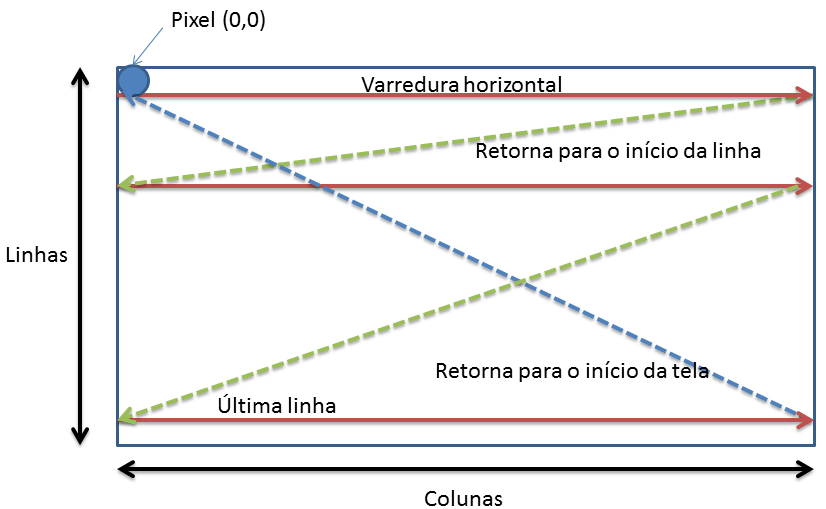
\includegraphics[width=0.9\textwidth]{img/controlador-vga-varredura-quadro-vga.png}
    \caption{Varredura do quadro. Autoria \cite{vga-sync}}
    \label{fig:vga-varredura}
\end{figure}

\begin{figure}[!h]
    \centering
    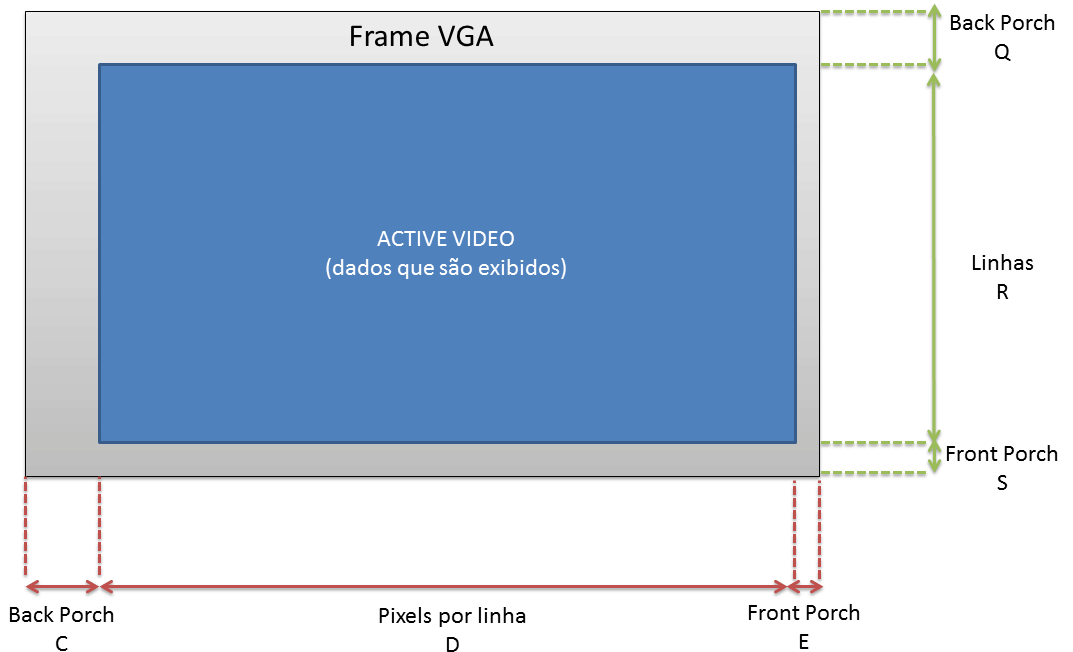
\includegraphics[width=0.9\textwidth]{img/controlador-vga-frame-vga.png}
    \caption{Frame VGA. Autoria \cite{vga-sync}}
    \label{fig:vga-frame}
\end{figure}

Numa tela de tamanho 800x600, com 72Hz de cadência (\emph{frame rate}) (50MHz de clock de pixel), os parâmetros são:

\begin{itemize}
    \item Horizontal
    \begin{itemize}
        \item \emph{Active Video}: 800px
        \item \emph{Front Porch}: 56px
        \item \emph{Back Porch}: 64px 
    \end{itemize}
    \item Vertical
    \begin{itemize}
        \item \emph{Active Video}: 600px
        \item \emph{Front Porch}: 37px
        \item \emph{Back Porch}: 23px
    \end{itemize}
\end{itemize}

O sincronismo horizontal é dado pelo seguinte diagrama. É determinado pelo sinal \emph{H\_SYNC}, que é ativado em nível lógico 0 e indica que uma linha foi finalizada e que a próxima será iniciada. O tempo necessário para esta resolução é equivalente ao tempo de varredura de 120 pixels.

\begin{figure}[!h]
    \centering
    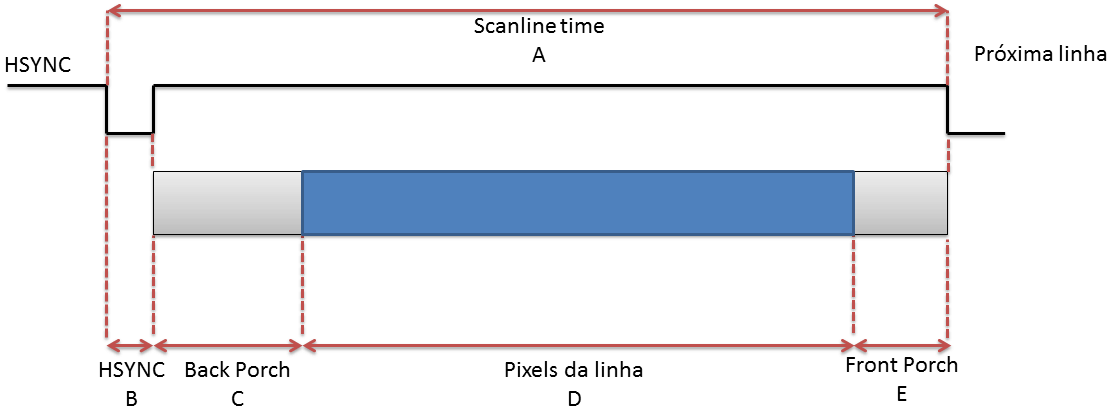
\includegraphics[width=0.9\textwidth]{img/controlador-vga-sincronizacao-horizontal-frame.png}
    \caption{Sincronismo horizontal do frame VGA. Autoria \cite{vga-sync}}
\end{figure}

O sincronismo vertical é dado pelo seguinte diagrama. É determinado pelo sinal \emph{V\_SYNC}, que é ativado em nível lógico 0 e indica que um quadro foi finalizado e que o próximo será iniciado. O tempo necessário para esta resolução é equivalente ao tempo de varredura de 6 pixels.

\clearpage

\begin{figure}[!h]
    \centering
    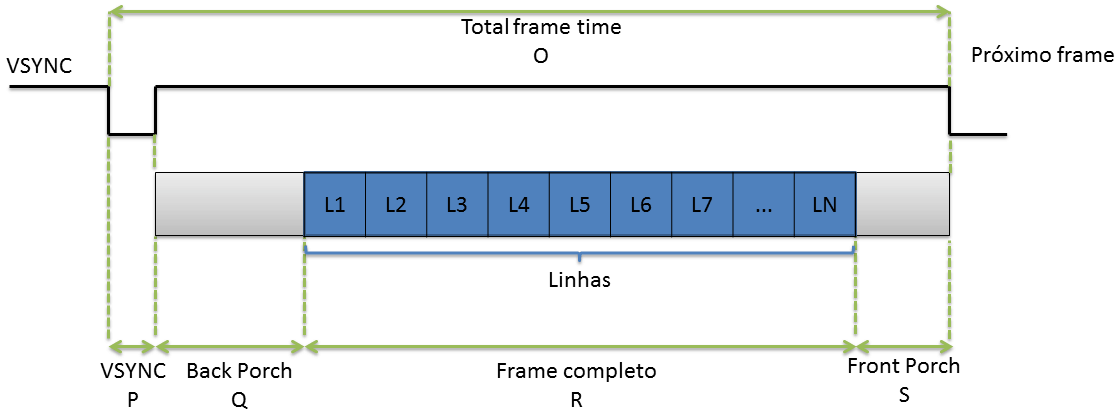
\includegraphics[width=0.9\textwidth]{img/controlador-vga-sincronizacao-vertical-frame.png}
    \caption{Sincronismo vertical do frame VGA. Autoria \cite{vga-sync}}
\end{figure}

A Figura \ref{fig:vga-frame-sync} apresenta a relação dos sinais de sincronismo para a exibição de um quadro.

\begin{figure}[!h]
    \centering
    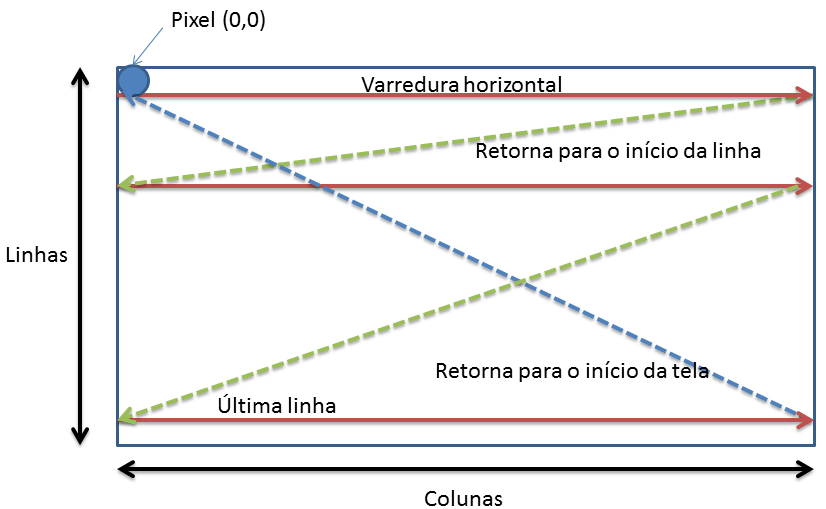
\includegraphics[width=0.9\textwidth]{img/controlador-vga-varredura-quadro-vga.png}
    \caption{Varredura do quadro. Autoria \cite{vga-sync}}
    \label{fig:vga-frame-sync}
\end{figure}

O \emph{kit Nexys2} contém um conector (DB15) para o cabo VGA. O controle de cor é dado de maneira analógica, como apresenta a figura a seguir. Para as componentes vermelha e verde, há 3 \emph{bits}, e para a azul, 2 \emph{bits} (uma vez que o olho humano é menos sensível aos níveis desta cor).

\clearpage

\begin{figure}[!h]
    \centering
    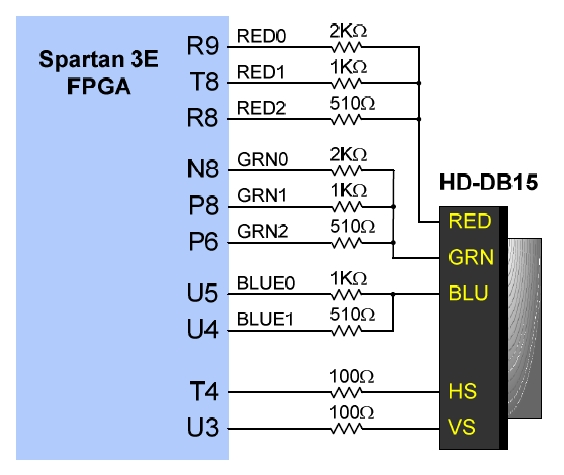
\includegraphics[width=0.5\textwidth]{img/rgb.jpg}
    \caption{Circuito de conexão com cabo VGA do kit Nexys2}
\end{figure}

\begin{figure}[!h]
    \centering
    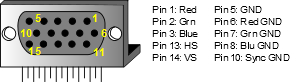
\includegraphics[width=0.6\textwidth]{img/VGA_Connector.jpg}
    \caption{Pinos do conector DB15}
\end{figure}

O anexo \ref{subsec:vga_controller} apresenta o código \emph{VHDL} da implementação. O circuito é responsável por gerar os pulsos de sincronismo vertical e horizontal, retornar o índice da linha e da coluna sendo processadas e o indicador de que está na região ativa do \emph{frame}.

%----------------------------
\subsection{Gerador gráfico}
\label{subsec:graphic-gen}
A função desta implementação é posicionar os elementos na tela. O quadro é separado em 6 regiões principais, uma para cada número sorteado. Cada uma dessas regiões é separada em 2 sub-regiões, uma para a dezena e outra para a unidade do número. A figura a seguir exemplifica a grade de posições.

\clearpage

\begin{figure}[!h]
    \centering
    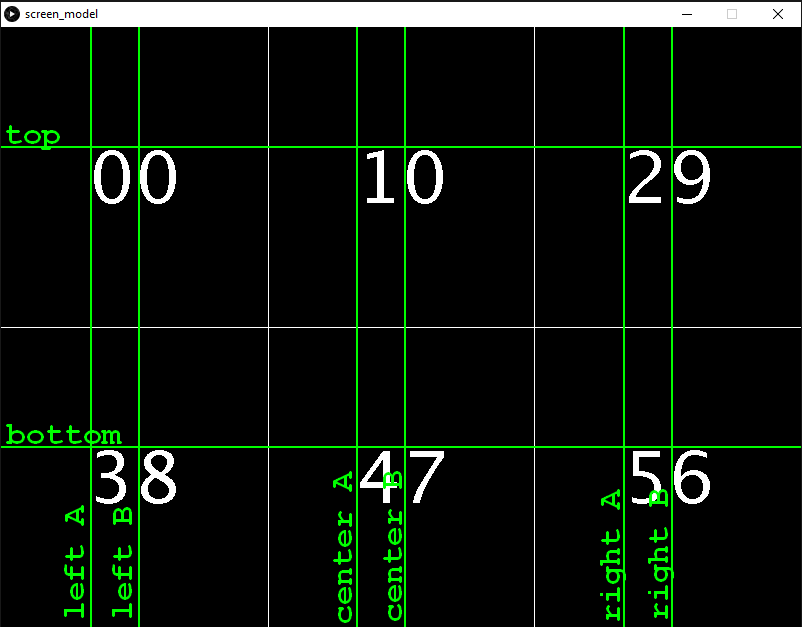
\includegraphics[width=0.65\textwidth]{img/pontos-tela.png}
    \caption{Posição dos números na tela.}
\end{figure}

Cada número sorteado é armazenado em uma memória de sinais VHDL. Os números são buscados na memória ROM (tópico \ref{subsec:font-rom}), onde estão decompostos em forma tipográfica, e são posicionados em ordem de sorteio.

O anexo \ref{subsec:vga_pixel_gen} apresenta o código \emph{VHDL} da implementação.

%----------------------------

\subsection{Fonte tipográfica}
\label{subsec:font-rom}
O circuito tem como base uma memória com os caracteres em forma tipográfica, de tamanho 39x57 pixels cada. Os 10 dígitos (0...9) ocupam 22.230 bits.

O desenho tipográfico dos caracteres foi extraído através de um programa feito em linguagem Processing \cite{p5}. O anexo \ref{subsec:processing} apresenta o código do extrator de caractere.

A função básica do circuito é retornar um vetor do tipo \emph{std\_logic\_vector} correspondente ao endereço solicitado. O gerador gráfico (tópico \ref{subsec:graphic-gen}) requisita linha a linha de um determinado caractere a fim de desenhá-lo por completo na tela.
%----------------------------

\subsection{Sorteio dos números}
O módulo que cuida do sorteamento se encontra no anexo ~\ref{subsec:sorteador} e reúne grande parte dos outros módulos. Quando um certo botão é apertado é utilizado o módulo de \textit{debounce}, o qual também faz com que a FSM avance de estado, além de receber um novo valor randômico. O módulo \textit{millis} é usado para fazer a troca de qual dos displays é ligado, juntamente com os módulos \textit{display7seg} e \textit{messages}. 

Embora reúna outros códigos, ainda não é o arquivo mais alto da hierarquia, ele controla o display, mas em seu port existe três saídas, a primeira é a unidade do valor sorteado, a segunda é a dezena do valor sorteado, e a terceira saída é um índice de qual estado a máquina se encontra. 

A máquina de estados é representada na figura \ref{fig:fsmsort}.

\begin{figure}[!h]
    \centering
    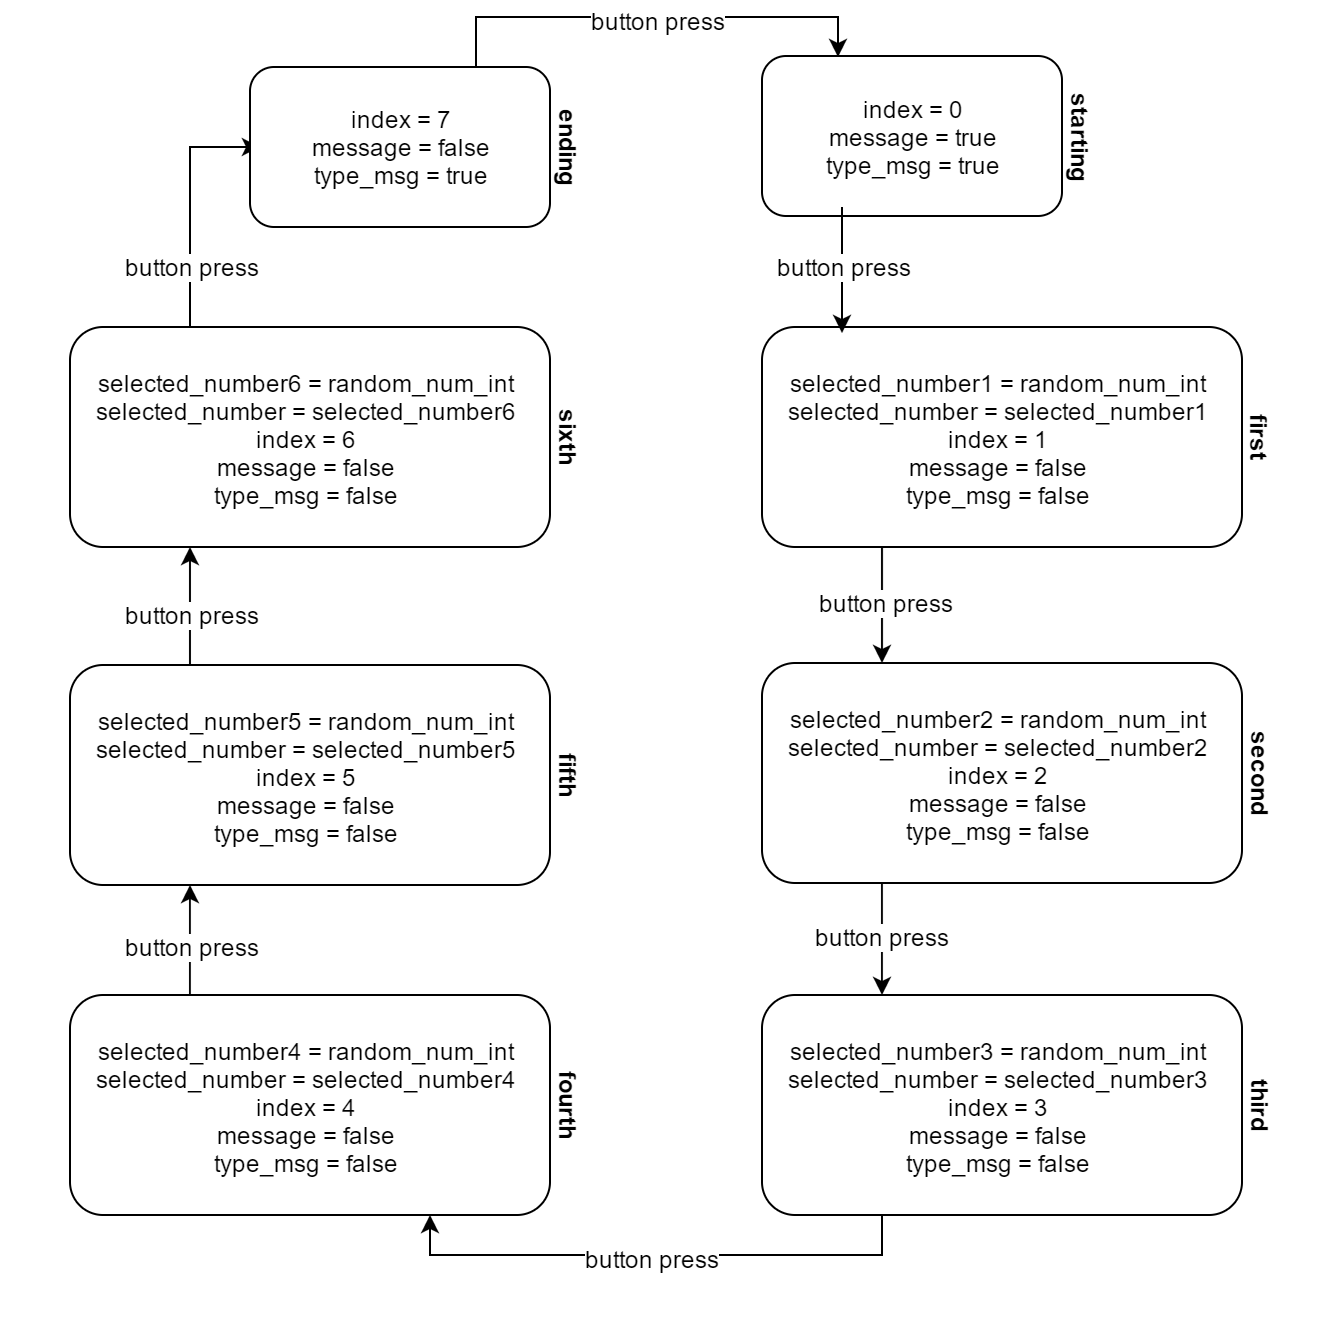
\includegraphics[width=0.98\textwidth]{img/sorteador-fsm.png}
    \caption{Diagrama de estados do sorteio}
    \label{fig:fsmsort}
\end{figure}

%----------------------------

\subsection{Tratamento de ``bounce`` para botão}
Para evitar acionamentos indesejados, é necessário tratar os sinais do botão na região de \emph{bouncing} (trepidação mecânica).

O \emph{design} para esta etapa é baseado no artigo \cite{debouncing-guide}, e visa tratar as trepidações tanto no pressionamento quando na liberação do botão tipo \emph{pushbutton} (botão de sorteio).

\begin{figure}[!h]
    \centering
    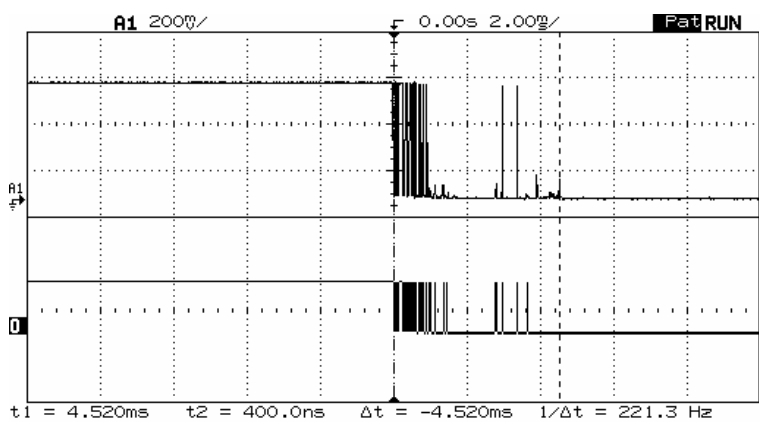
\includegraphics[width=0.8\textwidth]{img/debouncing_exemplo.jpg}
    \caption{Exemplo de trepidação de chaves mecânicas. Autoria \cite{debouncing-guide}}
    \label{fig:debouncing-ex}
\end{figure}

A implementação se trata de uma máquina de estados finitos (FSM, sigla em inglês). A Figura \ref{fig:debouncing-fsm} exemplifica seu diagrama de estados, onde:

\begin{itemize}
    \item in: entrada
    \item out: saída
    \item timer: tempo (em ms) de espera
    \item normal: nível lógico da chave quando não pressionada
    \item not normal: nível lógico da chave quando pressionada
\end{itemize}

\begin{figure}[!h]
    \centering
    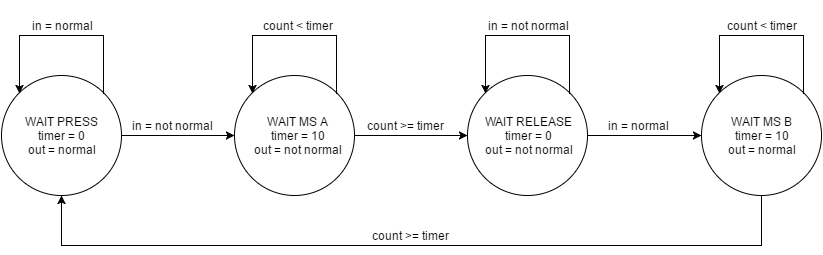
\includegraphics[width=1.0\textwidth]{img/fsm_debounce_sw.png}
    \caption{Diagrama de estados da FSM}
    \label{fig:debouncing-fsm}
\end{figure}

Os botões do \emph{kit} (Figura \ref{fig:nexys2_bots}) têm como nível normal o valor 0 (estão conectados ao terra), porém a equipe decidiu fazer este componente sendo genérico (opera com botões de nível normal 0 ou 1).

\begin{figure}[!ht]
    \centering
    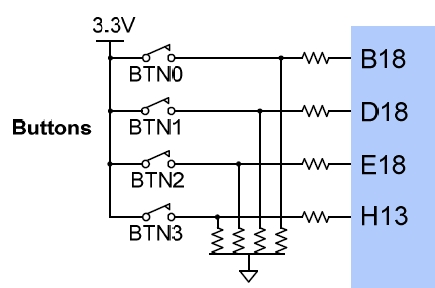
\includegraphics[width=0.4\textwidth]{img/nexys2_bots.jpg}
    \caption{Circuito de botões do \emph{kit Nexys 2}}
    \label{fig:nexys2_bots}
\end{figure}

O princípio de funcionamento é:
\begin{itemize}
    \item Aguardar pressionamento do botão
    \item Quando pressionado, aguardar 10ms (tempo de trepidação)
    \item Aguardar liberação do botão
    \item Quando liberado, aguardar 10ms (tempo de trepidação)
    \item Aguardar novo pressionamento
\end{itemize}

O anexo \ref{subsec:debounce-sw} apresenta o código \emph{VHDL} da implementação.

%----------------------------

\subsection{Mensagens e Display 7 Segmentos}
O display de 7 segmentos pode atuar de duas formas, primeiramente mostrando as mensagens inicial e final, ou mostrando os números sorteados. A variável que faz essa seleção esta presente no componentes \textit{sorteador} e é nomeada \textit{type\_seg}. Quando esta possui o valor \textit{true} será mostrado no display as mensagens, e os números quando for \textit{false}.

Tanto o módulo de mensagens quanto o de números recebem como entrada um identificador numérico que é convertido para \textit{std\_logic\_vector} de 7 bits. O qual é uma sequência que é convertida para o display de 7 segmentos. Essa sequência é no formato de "GFEDCBA" sendo que cada letra representa um dos segmentos, como mostrado na figura \ref{fig:disp}.

O código de tradução do display para as mensagens se encontra no anexo  ~\ref{subsec:message} e para os números em  ~\ref{subsec:disp7seg}.

\clearpage

\begin{figure}[!h]
    \centering
    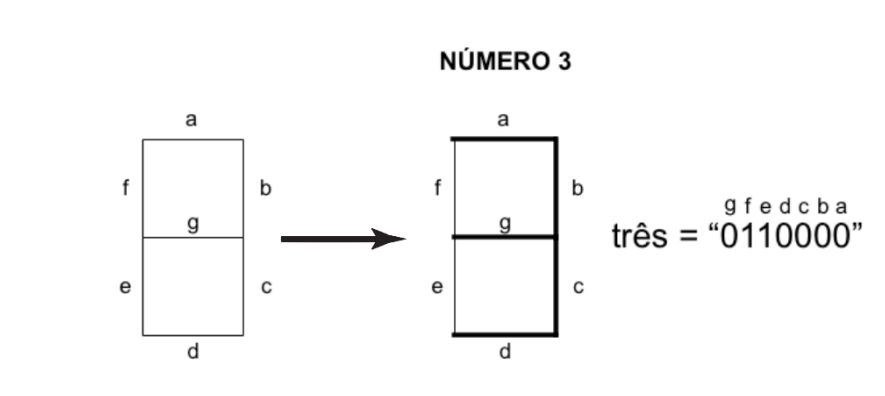
\includegraphics[width=0.7\textwidth]{img/disp.png}
    \caption{Tradução para o display de 7 segmentos}
    \label{fig:disp}
\end{figure}

%----------------------------

\subsection{Relógio}
Alguns componentes do projeto operam com contadores cuja a base de tempo é múltipla de 1ms. Assim, implementou-se o relógio \emph{``millis``}, cuja função é dividir o \emph{clock} de entrada de forma que sua saída seja uma onda quadrada cujo período é de 1ms.

Sua forma de operação é, basicamente, inverter seu estado a cada 0,5ms, tendo como base o oscilador do \emph{kit}, que é de 50MHz.

O anexo \ref{subsec:millis} apresenta o código \emph{VHDL} da implementação.
%----------------------------

\subsection{Gerador Pseudorrandômico}
Parte do desafio é cria uma forma de geração de números aleatórios, e para isso foi usado o método de \textit{registrador de deslocamento com realimentação linear}(LFSR) como ilustrado na figura \ref{rand}. Esse gerador utiliza 6 flip-flops, gerando então 64 números aleatórios, porém o valor só é atualizado na saída caso for diferente de 0 e menor ou igual a 60. O polinômio característico dessa geração é:

\begin{equation}
    N_{out} = 1 + x^5 + x^6
\end{equation}

\begin{figure}[!h]
    \centering
    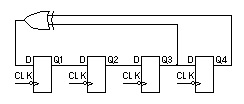
\includegraphics[width=0.7\textwidth]{img/lf.jpg}
    \caption{LFSR}
    \label{rand}
\end{figure}

O código implementado se encontra no anexo  ~\ref{subsec:random}.

\clearpage
%-------------------------------------------------------------
\section{Simulações}
%----------------------------
\subsection{Relógio}

O anexo \ref{subsec:tb_millis} apresenta o código \emph{VHDL} do \emph{testbench}, cujo objetivo é analisar o tempo entre as bordas de subida e também o \emph{reset}.

Abaixo, o diagrama temporal do \emph{testbench}.

\begin{figure}[!h]
    \centering
    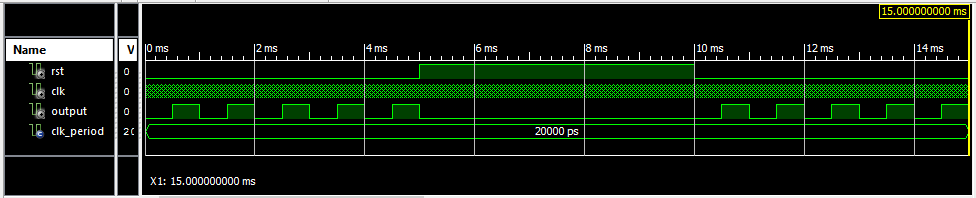
\includegraphics[width=1.0\textwidth]{img/tb_millis.png}
    \caption{Diagrama temporal do testbench do relógio.}
\end{figure}

Abaixo, verificação do tempo entre duas bordas de subida consecutivas: \begin{equation}
    1.499,99\mu s - 499,99\mu s = 1.000\mu s = 1ms
\end{equation}

\begin{figure}[!h]
    \centering
    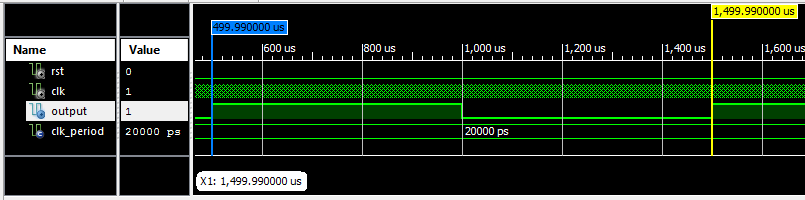
\includegraphics[width=1.0\textwidth]{img/tb_millis_zoom_1s.png}
    \caption{Verificação do relógio ``millis``.}
\end{figure}

\subsection{Debounce}

O anexo \ref{subsec:tb_debounce} apresenta o código \emph{VHDL} do \emph{testbench}, cujo objetivo é simular o componente frente à uma trepidação.

Abaixo, o diagrama temporal do \emph{testbench}.

\clearpage

\begin{figure}[!h]
    \centering
    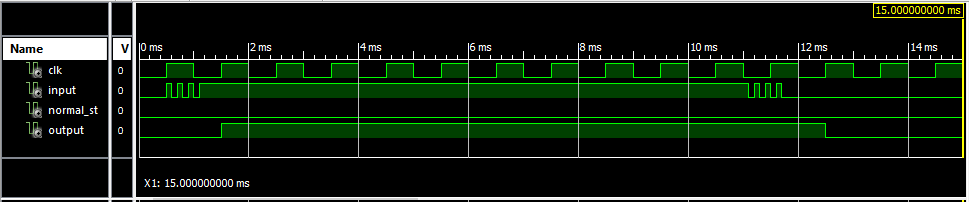
\includegraphics[width=1.0\textwidth]{img/tb_debounced_sw_NS0.png}
    \caption{Diagrama temporal do testbench do debounce.}
\end{figure}

\subsection{Random}

O anexo \ref{subsec:tb_random} apresenta o código \emph{VHDL} do \emph{testbench}, cujo objetivo é simular o componente random com o estimulo do clock.

Abaixo, o diagrama temporal do \emph{testbench}.
\begin{figure}[!h]
    \centering
    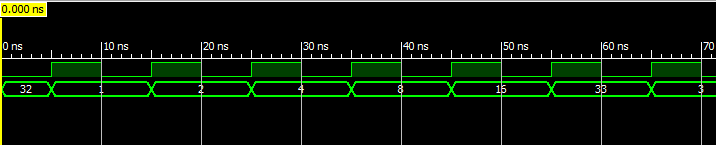
\includegraphics[width=1.0\textwidth]{img/tb_random.PNG}
    \caption{Diagrama temporal do testbench do random.}
\end{figure}


\clearpage
%-------------------------------------------------------------
\begin{thebibliography}{}
%----------------------------
\bibitem{vga-sync}
Controlador VGA,
\\\texttt{http://www.embarcados.com.br\/controlador-vga-parte-1/}
%----------------------------
\bibitem{p5}
Processing,
\\\texttt{https://processing.org/}
%----------------------------
\bibitem{debouncing-guide} 
A [!h] to Debouncing,
\\\texttt{http://www.eng.utah.edu/\~{}cs5780/debouncing.pdf}
%----------------------------
\end{thebibliography}

\clearpage
%-------------------------------------------------------------
\section{Anexos}
%----------------------------
\subsection{loteria.vhd}
\label{subsec:loteria}
\inputminted{vhdl}{code/loteria.vhd}
%----------------------------
\subsection{vga\_controller.vhd}
\label{subsec:vga_controller}
\inputminted{vhdl}{code/vga_controller.vhd}
%----------------------------
\subsection{vga\_pixel\_gen.vhd}
\label{subsec:vga_pixel_gen}
\inputminted{vhdl}{code/vga_pixel_gen.vhd}
%----------------------------
\subsection{font\_rom.vhd}
\label{subsec:font_rom}
\inputminted{vhdl}{code/font_rom.vhd}
%----------------------------
\subsection{sorteador.vhd}
\label{subsec:sorteador}
\inputminted{vhdl}{code/sorteador.vhd}
%----------------------------
\subsection{debounced\_sw.vhd}
\label{subsec:debounce-sw}
\inputminted{vhdl}{code/debounced_sw.vhd}
%----------------------------
\subsection{display7seg.vhd}
\label{subsec:disp7seg}
\inputminted{vhdl}{code/display7seg.vhd}
%----------------------------
\subsection{messages.vhd}
\label{subsec:message}
\inputminted{vhdl}{code/messages.vhd}
%----------------------------
\subsection{millis.vhd}
\label{subsec:millis}
\inputminted{vhdl}{code/millis.vhd}
%----------------------------
\subsection{random.vhd}
\label{subsec:random}
\inputminted{vhdl}{code/random.vhd}


%----------------------------
\subsection{tb\_millis.vhd}
\label{subsec:tb_millis}
\inputminted{vhdl}{code/tb_millis.vhd}
%----------------------------
\subsection{tb\_debounced\_ws.vhd}
\label{subsec:tb_debounce}
\inputminted{vhdl}{code/tb_debounced_sw.vhd}
%----------------------------
\subsection{tb\_random.vhd}
\label{subsec:tb_random}
\inputminted{vhdl}{code/tbrandom.vhd}
%----------------------------
\subsection{char\_extractor.pde}
\label{subsec:processing}
\inputminted{java}{code/char_extractor.pde}
%----------------------------


\end{document}
